\documentclass[12pt]{article}
\usepackage[margin=1in]{geometry}
\geometry{letterpaper}
\usepackage{doc}
\usepackage{arydshln}
\usepackage{url}
\usepackage{graphicx}
\usepackage[none]{hyphenat}
\usepackage{epstopdf}
\usepackage[titletoc,toc,title]{appendix}
\usepackage{amssymb}
\usepackage{pdfpages}
\usepackage{acronym}
\usepackage{verbatim}
\usepackage{enumerate}
\usepackage{fancyhdr}
\usepackage{wrapfig}
\usepackage{subcaption}
\usepackage{amsmath}
\usepackage[nottoc, notlof, notlot]{tocbibind}
\usepackage[colorlinks=true, linkcolor=blue]{hyperref}

\DeclareGraphicsRule{.tif}{png}{.png}{`convert #1 `dirname #1`/`basename #1 .tif` .png}
\newcommand\norm[1]{\left\lVert#1\right\rVert}
% Header
\pagestyle{fancy}
\renewcommand{\headrulewidth}{0.4pt}
\lhead{\textsc{Companion}}
\rhead{Robot Security}

\begin{document}
\newcommand{\HRule}{\rule{\linewidth}{0.5mm}}
\begin{titlepage}
\begin{center}

\includegraphics[width=0.25\textwidth]{./logo.png}~\\[0.3cm]

\textsc{\large University of Toronto}\\[0.5cm]
\HRule \\[0.2cm]
{ \textsc{\large Companion}\\
\LARGE \bfseries Robot Security \\[0.2cm] }
\HRule \\[0.5cm]

\textsc{\large ECE1778 Winter 2015}\\
{Creative Applications for Mobile Devices}\\[0.5cm]
\textbf{\large Wei Hao Chang} \texttt{Apper}\\
\textbf{\large Alexander Hong} \texttt{Programmer}\\

\includegraphics[width=0.65\textwidth]{./companion.png}~\\
\vfill
{\large \today}

\end{center}
\end{titlepage}
\pagebreak
\tableofcontents
\pagebreak
%\listoffigures
%\pagebreak
%\listoftables
%\pagebreak

% Calibration
\topskip0pt
\vspace*{\fill}
\renewcommand{\abstractname}{Executive Summary}
\abstract
Your own personal robot is here to serve and protect you! This document outlines the design of an Android application for an assistive security robot. The application connects to a LEGO Mindstorm EV3 Brick to control the robot's mobile base and another smartphone as the face for the robot. The robot follows the user as a personal body guard and is able to respond to the user's need for help. With 3 alarm systems, the robot is able to ward off unwanted individuals near the user. Moreover, the robot has her own personality and can interact with facial expressions to the user.
\vfill
\begin{center}\texttt{\LARGE Word Count: 2,456}\end{center}
\begin{center}
\texttt{Source Code:} \url{https://github.com/thealexhong/companion/}
\end{center}
\vspace*{\fill}
\pagebreak

\section{Introduction}
\subsection{Problem}
Recent survey shows that there are about 31 million total crimes reported annually. Thefts, assaults, and sexual assaults makes up 76\% of the total crime and were commonly performed between the hours between 6 pm to 4 am [1]. In U.S., 37\% of the people do not feel safe walking alone at night in their neighborhood [2], and 38\% of students felt unsafe when travelling from their campus to their accommodation at night. According to \textit{Crime-Statistics Against Women}, 36 cases of sexual assault and rape against women happen every hour [3]. 

In Canada, the Angus Reid Poll shows 65\% of females surveyed experience fear or feel concerned for their safety when walking alone at night. Although women continue to be the primary target of violent offences in Canada, only 13\% carry a protection device, such as a flashlight or panic alarm [4]. Even with the high nighttime crime rate, there have not been any effective defensive devices in the market that could ward off potential attackers. Current solutions do not provide immediate help, and are not always accessible. Hence, the goal of this application is to provide a smarter solution that can allow individuals to feel safer and more empowered, particularly in situations when they find themselves walking alone after hours.

\subsection{Objective}
Our aim is to combine the traditional methods of personal protections with robotics and mobile application to propose a novel solution to better protect any late night walkers. The objective of the project is to develop an application that uses a smartphone as a central control and communication unit to interact with an autonomous robot. By having a smartphone paired up with the robot, the robot is able to follow the user closely, and perform alarm actions upon trigger. These alarm actions (i.e. display alert, siren alert, and robot action alert) can be trigger manually or autonomously to ward off potential attackers.

\section{Overall Design}
The overall design of our product combines both software (i.e., the mobile application) and hardware (i.e., robot) to work together in harmony to achieve our objectives. The following section describes both our software and hardware design.

\subsection{Software Design}
The software design of Robot Security comprises of 2 major subsystems: (i) \textit{User's Phone} and (ii) \textit{Companion Robot}, Figure~\ref{system}.

\begin{figure}[!htbp]
    \centering
    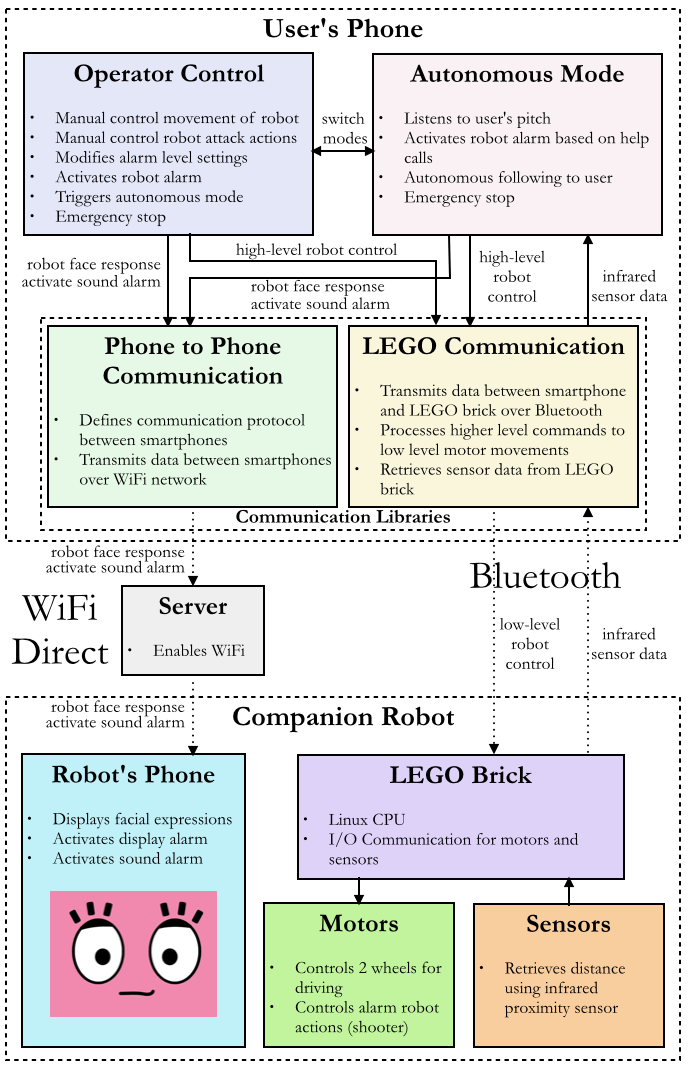
\includegraphics[width=0.8\textwidth]{system.png}
    \caption{System Diagram of Robot Security}
    \label{system}
\end{figure}

Our application requires 2 smartphones. When launching the application, the user is presented with two modes: (i) \texttt{Connect}, and (ii) \texttt{Launch Companion}, Figure~\ref{home}. \texttt{Connect} will connect the present phone to the robot and another smartphone in the same WiFi network. The phone in this setting will operate as the \textit{User's Phone}. \texttt{Launch Companion} will launch the robot's face and the corresponding phone under this setting will act as the robot's face (mounted to the robot). This is represented as the \textit{Robot's Phone} block in Figure~\ref{system}.

\begin{figure}[!htbp]
    \centering
    
\includegraphics[width=0.3\textwidth]{home.png}
    \caption{Home Screen of Robot Security}
    \label{home}
\end{figure}

\subsubsection{User's Phone Subsystem}
The User's Phone is the central control system of the robot. It's main purpose is to allow the user to control the robot and respond to the user's cry for help. This is accomplished through \textit{Operator Control} mode and \textit{Autonomous Mode} respectively. 

\paragraph{Operator Control}

In \textit{Operator Control} mode, the user is able to manually control the robot through primitive actions such as move forward, backward, turn left, and turn right. In addition, the user may also manually control the robot to attack using a shooter. The \textit{Operator Control} mode screen is illustrated in Figure~\ref{control}.

\begin{figure}[!htbp]
    \centering
    \begin{subfigure}[b]{0.45\textwidth}
    \centering
    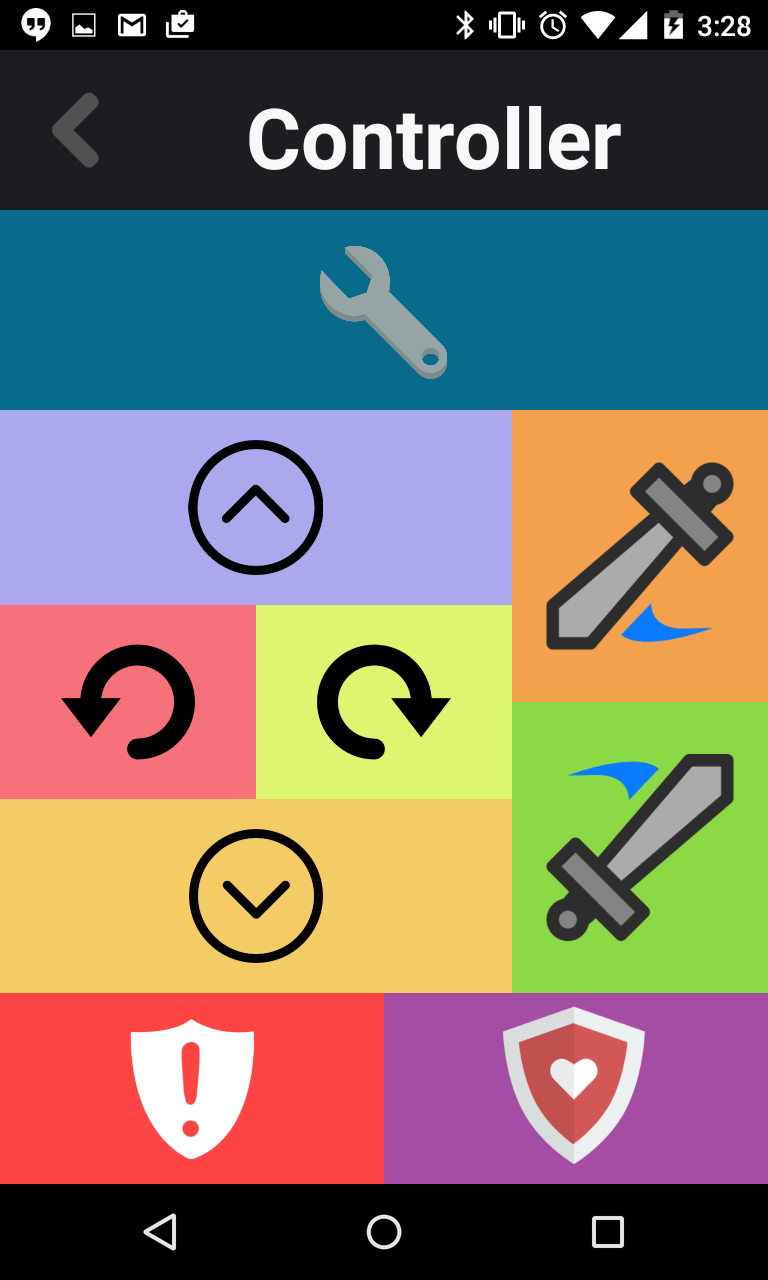
\includegraphics[width=0.75\textwidth]{controller.png}
    \caption{Control Screen of Robot Security}
    \label{control}
    \end{subfigure}
    \begin{subfigure}[b]{0.45\textwidth}
    \centering
    
\includegraphics[width=0.75\textwidth]{settings.png}
    \caption{Alarm Setting Screen of Robot Security}
    \label{settings}
    \end{subfigure}\\~\\
    \centering
    \begin{subfigure}[b]{0.45\textwidth}
    \centering
    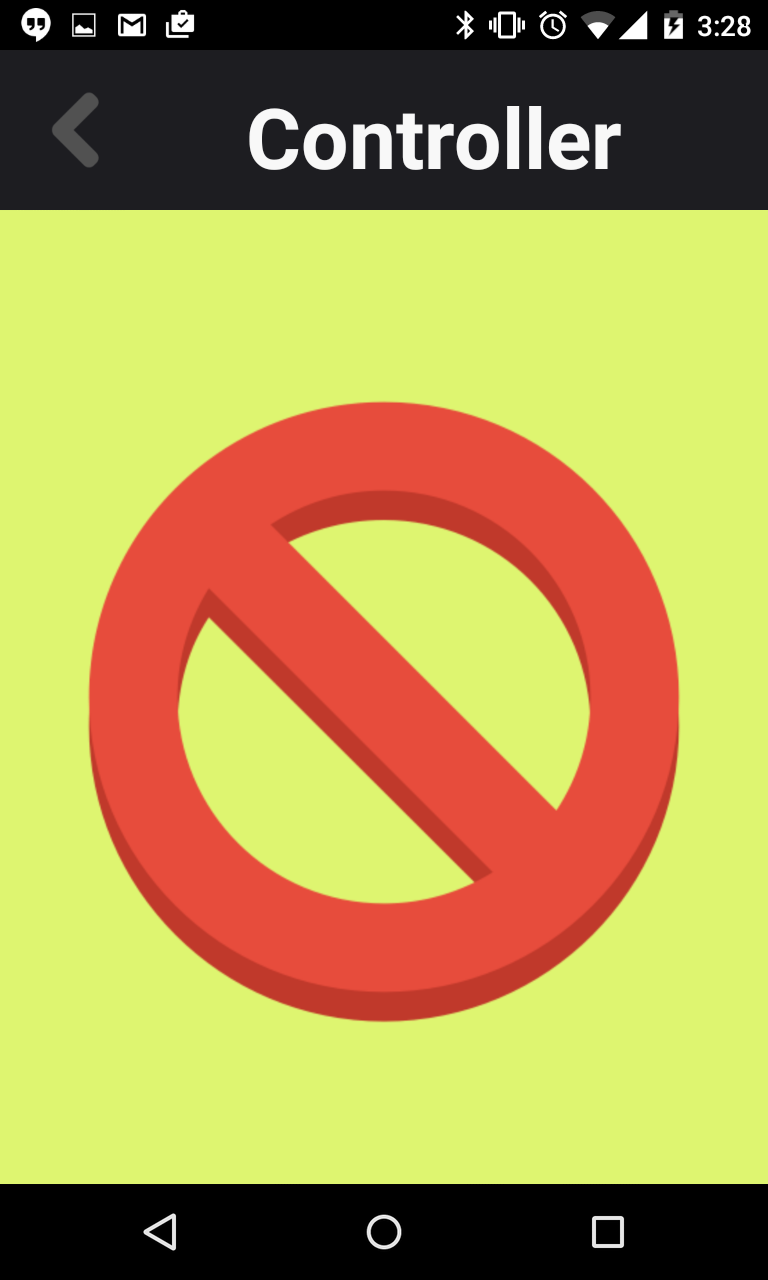
\includegraphics[width=0.75\textwidth]{stop.png}
    \caption{Emergency Stop Button}
    \label{stop}
    \end{subfigure}
    \begin{subfigure}[b]{0.45\textwidth}
    \centering
    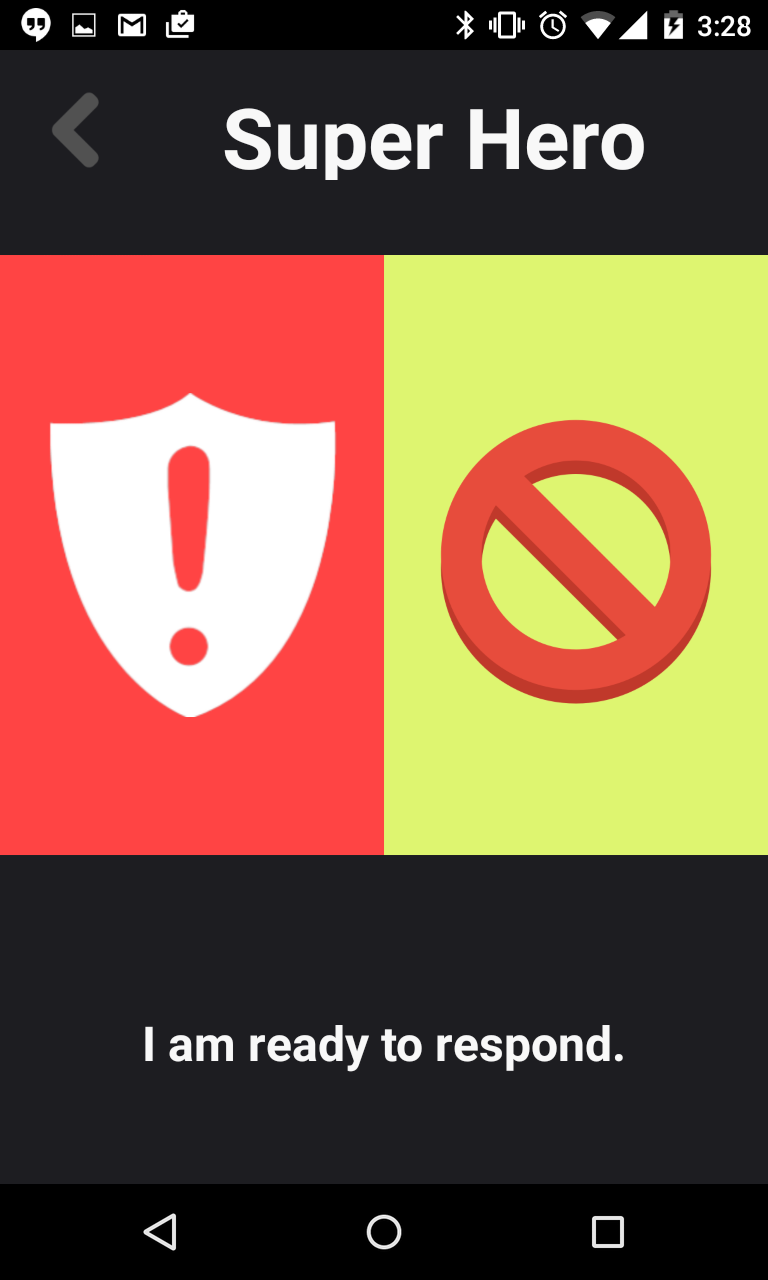
\includegraphics[width=0.75\textwidth]{superhero.png}
    \caption{Autonomous Mode Screen}
    \label{superhero}
    \end{subfigure}
    \caption{Screens of Robot Security}
    \label{screens}
\end{figure}
\pagebreak
In this mode, the user may also change the 3 alert level settings: (i) \textit{Display Alert}, (ii) \textit{Siren Alert}, and (iii) \textit{Robot Action Alert}. These alert levels may be adjusted in the settings menu of our application, Figure~\ref{settings}. \textit{Display Alert} activates an alert angry face, Figure~\ref{facealert}. During normal operations, the robot expresses various facial expressions depending on the scenario, Figure~\ref{facerobot}. \textit{Display Alert} activates the alert angry face to ward off potential attackers. \textit{Siren Alert} activates a verbal warning follow by a loud siren when the robot is in alert mode to simulate public authority. Lastly, \textit{Robot Action Alert} activates a robot action to ward off potential attackers. In the current revision of the application, the action is set to continuously move the robot forward and shoot balls from its shooter.

The user may also manually activate alert mode. This will activate the alerts set in the setting menu. Whenever the robot is in alert mode, the user's phone is presented with an emergency stop button, Figure~\ref{stop}. Pressing this button will stop all robot alerts and the robot will return back to a neutral state.

\begin{figure}[!htbp]
    \centering
    \begin{subfigure}[b]{0.23\textwidth}
    \centering
    
\includegraphics[width=\textwidth]{4.png}
    \caption{Admirable}
    \label{like}
    \end{subfigure}
    \begin{subfigure}[b]{0.23\textwidth}
    \centering
    
\includegraphics[width=\textwidth]{5.png}
    \caption{Neutral}
    \label{neutral}
    \end{subfigure}
    \begin{subfigure}[b]{0.23\textwidth}
    \centering
    
\includegraphics[width=\textwidth]{3.png}
    \caption{Neutral left}
    \label{neutralleft}
    \end{subfigure}
    \begin{subfigure}[b]{0.23\textwidth}
    \centering
    
\includegraphics[width=\textwidth]{6.png}
    \caption{Neutral right}
    \label{neutralright}
    \end{subfigure}\\~\\
    \begin{subfigure}[b]{0.23\textwidth}
    \centering
    
\includegraphics[width=\textwidth]{1.png}
    \caption{Angry}
    \label{angry}
    \end{subfigure}
    \begin{subfigure}[b]{0.23\textwidth}
    \centering
    
\includegraphics[width=\textwidth]{7.png}
    \caption{Sad}
    \label{sad}
    \end{subfigure}
    \begin{subfigure}[b]{0.23\textwidth}
    \centering
    
\includegraphics[width=\textwidth]{8.png}
    \caption{Sleepy}
    \label{sleepy}
    \end{subfigure}
    \begin{subfigure}[b]{0.23\textwidth}
    \centering
    
\includegraphics[width=\textwidth]{9.png}
    \caption{Surprised}
    \label{surprised}
    \end{subfigure}\\~\\
    \begin{subfigure}[b]{0.45\textwidth}
    \centering
    
\includegraphics[width=\textwidth]{2.png}
    \caption{Happy}
    \label{happy}
    \end{subfigure}
    \begin{subfigure}[b]{0.45\textwidth}
    \centering
    
\includegraphics[width=\textwidth]{10.png}
    \caption{Face Alert}
    \label{facealert}
    \end{subfigure}
    \caption{Face of Robot Security}
    \label{facerobot}
\end{figure}

\paragraph{Autonomous Mode}
In \textit{Autonomous Mode}, the robot will follow the user using a Proportional-Derivative (PD) controller. Using the data from an infrared sensor on the robot, the autonomous controller on the user's phone sends high-level robot commands to move the robot in the appropriate direction. \textit{Autonomous Mode} also includes a pitch detector by converting sound signals to the frequency domain and analyzing pitch level. When the user's pitch level is high enough (i.e., when the user screams), the robot is able to autonomously respond and activate its alert mode to protect the user. Again, the user is presented with an emergency stop button, Figure~\ref{superhero}.

\paragraph{Phone to Phone Communication}
The \textit{Phone to Phone Communication} library defines the communication protocols and functions for transmitting data over the WiFi network using WiFi Direct between user's phone and the robot's phone. This library is mainly used for receiving controls from the user to change the robot's facial expression, and activate \textit{Display Alert} and \textit{Siren Alert}. A \textit{Server} hosts WiFi service for phones to connect and communicate.

\paragraph{LEGO Communication}
The \textit{LEGO Communication} library defines functions for transmitting data between the user's phone and the LEGO Mindstorm EV3 Brick over Bluetooth. The library takes high-level robot commands from user's phone, and converts them into bytes for the \textit{LEGO Brick}. Commands such as forward, backward, etc. are considered as "high level commands". The library also converts low-level signals obtained from the brick and processes them into higher-level values. For example, the signal from the infrared sensor is processed into distance and angle values for \textit{Autonomous Mode} to understand.

\subsubsection{Companion Robot Subsystem}
The companion robot subsystem consists of the \textit{Robot's Phone}, and \textit{LEGO Brick}.

\paragraph{Robot's Phone}
The \textit{Robot's Phone} displays an array of facial expressions, Figure~\ref{facerobot}. The \textit{Robot's Phone} processes signals from the \textit{Phone to Phone Communication} module and responds with changing facial expressions, or activate alerts when appropriate. This module has the ability to activate the display alert and siren alert. The siren alert is activated by playing a loud siren sound in a loop.

\paragraph{LEGO Brick}
The \textit{LEGO Brick} processes low-level robot control (bytes) into motor actions. The \textit{LEGO Brick} controls the two wheels for driving the robot, and activates the robot shooter when action command is sent. Sensor data retrieved from the infrared sensor is also passed into the \textit{LEGO Brick} before being processed by the \textit{LEGO Communication} library.

\subsection{Hardware System}
Figure~\ref{hardware} shows a past revision of the robot. The robot consist of three servo motors, and one infrared sensor. Two servo motors are geared up and used for the movement of the robot to keep up with the walking speed on the user. The third servo motor is used for the robot shooter. The infrared sensor on the robot receives infrared signal from an infrared emitter to perform autonomous following. Furthermore, the robot can house the robot's phone to display facial expressions and alert.

\begin{figure}[!htbp]
    \centering
    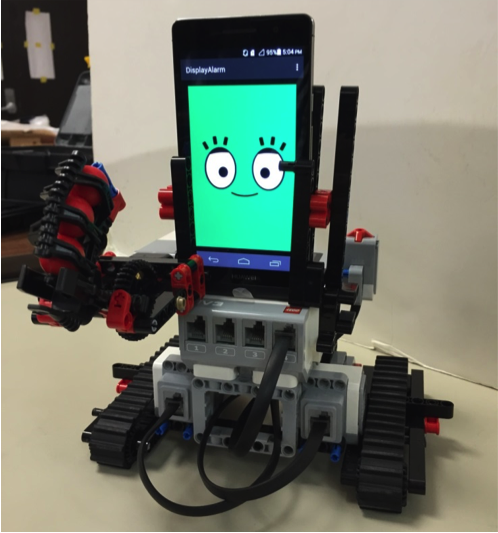
\includegraphics[width=0.5\textwidth]{hardware.png}
    \caption{Robot Security Hardware}
    \label{hardware}
\end{figure}

\section{Statement of Functionality}
Overall, the application successfully achieves the project objective; it enables remote control of the security robot, and performs alarm actions upon trigger. Furthermore, the robot autonomously follows the user. The specific successes, failures, and areas for improvements are discussed in the following section.

\subsection{User Interface / User Experience}
The UI design and UX was a success. The design was based on flat design, and optimize for simplicity to achieve user friendliness. Screenshots of the application is shown in Figure~\ref{screens}. This has been simplified from our previous UI design.

\subsection{Remote Control}
Our application has full remote control over the security robot. The user may send commands to the robot's LEGO Mindstorm EV3 Brick via Bluetooth to control the robot's movements. Multi-threading of different commands enabled users to use multi-touch to control the robot to do several actions at once (i.e., move and attack). The motor speed on the robot was greatly improved from earlier version by: (i) modifying the bytes being sent, and  (ii) gearing up the motors.

\subsection{Alert Actions}
When the user activates the robot alerts manually, or when the robot detects the user's high pitch (i.e., when the user screams), the robot activates alert mode. The 3 selected alert actions proved to be effective.

\begin{enumerate}
\item Display Alert: During normal operations, the robot will change its facial expression depending on the scenario. When alert mode is triggered, the robot will be fearful with its angry face to ward off potential attackers, Figure~\ref{facerobot}.
\item Siren Alert: The robot will announce a pre-programmed verbal warning via audio using robot's phone to warn the potential attacker before sounding the siren alarm.
\item Robot Action Alert: The robot will start shooting balls to ward off potential attacker after sounding the alarm.
\end{enumerate}

\subsection{Pitch Detection}
The designed pitch detection algorithm was tested to be accurate enough to tune a guitar. By transforming sound signals in frequency domain and analyzed for pitch levels, high pitch from the user to trigger alerts can be detected. The pitch detector was further optimized for user's scream (1000 Hz).

\subsection{Autonomous User Following}
The initial plan was to only use phone hardware to accomplish autonomous user following. Different approaches were attempted, but failed due to unreliable sensor readings. Firstly, waypoint navigation was attempted using GPS. However, GPS readings proved to be unreliable within operating distance of our application due to low resolution and high latency. Secondly, using Bluetooth signal strength as a distance feedback also proved to be unreliable as the signal strength has high variance. Lastly, using the phone's accelerometer and gyroscope for autonomous following proved to be difficult. The system was not robust enough to be able to function as intended.

This problem was solved using external infrared sensor/emitter pair. This solution proved to be the most robust for our application. The infrared emitter sends binary command to the receiver constantly to the robot to obtain the distance and angle of the signal. The controller then uses the signal angle, and signal distance for motor direction and speed. Moreover, a derivative control is used to further calculate the change of error to improve stability during following.

\section{Lessons Learned}
After completing this project, we are able to: (i) write the communication library to control the LEGO controller, while having the WiFi direct communicate between the two phones, (ii) use a frequency filter for sound triggering alarms, and (iii) design an autonomous following algorithm using infrared sensor information.
\subsection{User-Experience}
The user-experience is a critical factor in the design of this system, since multiple functions are involved for the control of the robot, we have learned to tackle the UX early on in the spiral 2. Hence the UI was greatly simplified for user friendliness.

\subsection{Software-Hardware Interface}
Interfacing with hardware components from software is always a challenging endeavor. However, we were able to establish the communication libraries early (i.e., \textit{LEGO Communication} library, \textit{Phone to Phone Communication} library) and use primitive functions to determine potential project improvements.

\subsection{Spiral Method} 
Utilising the spiral method was a highly effective strategy. It allowed us to set milestones and manage our goals to tackle on the more challenging problems in a relatively organized and manageable fashion.

\section{Contributions}
Both members played an equal role in the development on Robot Security. The following lists the individual contributions to the project.
\subsection{Wei Hao Chang}
\begin{itemize}
\item Designed and built all revisions of the hardware prototype
\item Designed and built the preliminary application user-interface layout
\item Designed and built preliminary WiFi direct, and voice trigger
\item Designed and built autonomous PD controller
\item Co-authored final presentation and report
\end{itemize}
\subsection{Alexander Hong}
\begin{itemize}
\item Designed and built all revisions of the application software
\item Designed and built the final application user-interface layout
\item Designed and built communication libraries between devices
\item Integrated WiFi direct, and voice trigger
\item Troubleshooted  issues with software and suggested improvements
\item Co-authored final presentation and report
\end{itemize}

\section{Apper Context}
To recap, the apper's background is in mechatronics and sensory design, and he has received M.A.Sc degrees in Mechanical Engineering. His research includes: hardware/software sensory design, and implementation of the intelligent perception for autonomous high-speed robotics applications. His field of knowledge is highly related to sensory system design for human assisting robotic applications using either autonomous or semi-autonomous controls.

In this project, there is a particular interest in the implementation and application of smartphones sensors with robotic technologies to perform human assisting applications. Throughout this project, the robot prototype, communication library, autonomous controller, and a mobile application were built for the security application. The application developed from this project demonstrate a practical implementation of good human robot interaction practices in design and further provides a valuable tool for prototyping and future commercial security robot implementations.

\section{Future Work}
As discussed in the Introduction, the goal of Robot Security is to accompany and protect late night walkers. Given the novelty of the application, a system such as Robot Security has potential for commercial success. However, the current application requires significant improvements to the performance for robustness, as well as testing with full-scale robot devices before it can be commercialized.
With more time and resources, there are several areas the application can benefit from improvements:
\begin{enumerate}
\item Apply to multiple robot platforms (e.g., drones)
\item Include speech and voice recognition for user voice commands
\item Include smart image processing for obstacle avoidance, object tracking, and object recognition
\item Be able to support cross-platform mobile devices
\end{enumerate}

\section*{References}
\begin{enumerate}
\begin{sloppypar}
\item M. Felson , E. Poulsen, ``Simple indicators of crime by time of day", International Journal of Forecasting, vol. 19, pp. 595-601, 2003
\item J, Stein. ``Majority of Canadian women feel unsafe walking at night", CNW, [Online] 2008, \url{http://www.newswire.ca/en/story/349535/majority-of-canadian-women-feel-unsafe-walking-at-night} Accessed:  22 January 2015).
\item Angie M. Tarighi, ``Crime-Statistics Against Women", Women’s Self-Defense Institute, [Online] 2014, \url{http://www.self-defense-mind-body-spirit.com/crime-statistics.html} (Accessed:  22 January 2015).
\item Andrew Dugan, ``In U.S., 37\% Do Not Feel Safe Walking at Night Near Home," Gallup, [Online] 2014, \url{http://www.gallup.com/poll/179558/not-feel-safe-walking-night-near-home.aspx} (Accessed:  22 January 2015).
\end{sloppypar}
\end{enumerate}

\end{document}